\documentclass{standalone}
\usepackage{tikz}
\usetikzlibrary{decorations.markings}

\tikzset{-node-/.style={decoration={
    markings,
    mark=at position #1 with {
        \draw[fill=green!60!black, line width=0.4] circle [radius=0.1];}},
    postaction={decorate}}}

\begin{document}
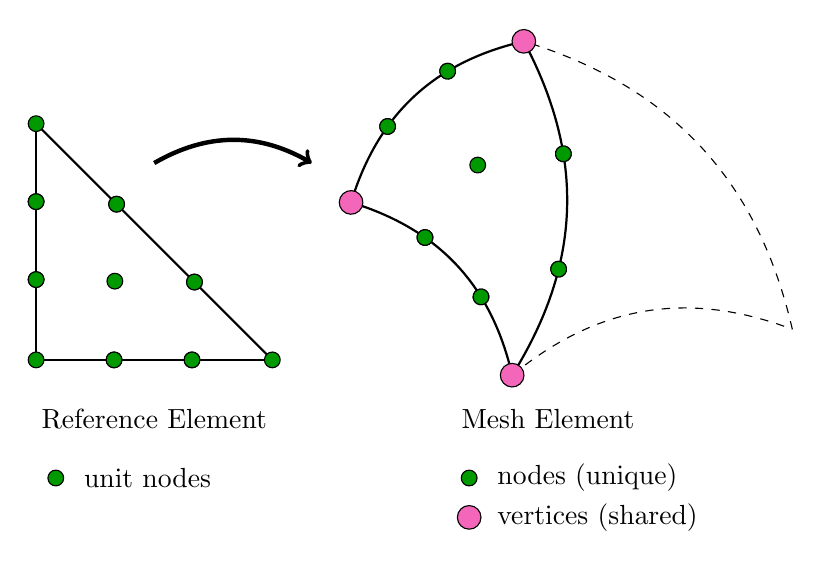
\begin{tikzpicture}
\draw [thick, -node-=.33,-node-=0.66] (0, 0) to (3, 0);
\draw [thick, -node-=.33,-node-=0.66] (3, 0) to (0, 3);
\draw [thick, -node-=.33,-node-=0.66] (0, 3) to (0, 0);
\draw [fill=green!60!black] (0, 0) circle [radius=0.1];
\draw [fill=green!60!black] (3, 0) circle [radius=0.1];
\draw [fill=green!60!black] (0, 3) circle [radius=0.1];
\draw [fill=green!60!black] (1, 1) circle [radius=0.1];

\draw [ultra thick,bend left,->] (1.5, 2.5) to (3.5, 2.5);

\begin{scope}[shift={(4, 2)},rotate=-47]
\draw [thick, -node-=.33,-node-=0.66] (0, 0) to [bend left] (3, 0);
\draw [thick, -node-=.33,-node-=0.66] (3, 0) to [bend right] (0, 3);
\draw [thick, -node-=.33,-node-=0.66] (0, 3) to [bend right] (0, 0);
\draw [dashed] (3, 0) to [bend left] (5, 3);
\draw [dashed] (5, 3) to [bend right] (0, 3);

\draw [fill=magenta!60] (0, 0) circle [radius=0.15];
\draw [fill=magenta!60] (0, 3) circle [radius=0.15];
\draw [fill=magenta!60] (3, 0) circle [radius=0.15];
\draw [fill=green!60!black] (0.75, 1.5) circle [radius=0.1];
\end{scope}

\node at (1.5, -0.5) [below] {Reference Element};
\draw [fill=green!60!black] (0.25, -1.5) circle [radius=0.1] 
    node [right] {~ unit nodes};
\node at (6.5, -0.5) [below] {Mesh Element};
\draw [fill=green!60!black] (5.5, -1.5) circle [radius=0.1] 
    node [right] {~ nodes (unique)};
\draw [fill=magenta!60] (5.5, -2) circle [radius=0.15] 
    node [right] {~ vertices (shared)};
\end{tikzpicture}
\end{document}
